\documentclass[conference]{IEEEtran}
\IEEEoverridecommandlockouts
% The preceding line is only needed to identify funding in the first footnote. If that is unneeded, please comment it out.
\usepackage{cite}
\usepackage{amsmath,amssymb,amsfonts}
\usepackage[labelfont=bf]{caption}
\usepackage{graphicx}
\usepackage{subcaption}
\usepackage{textcomp}
\usepackage[bottom]{footmisc}
\usepackage{amsmath}
\usepackage{xcolor}
\usepackage{float}
\usepackage{algorithm}
\usepackage[noend]{algpseudocode}
\DeclareMathOperator{\E}{\mathbb{E}}
\def\BibTeX{{\rm B\kern-.05em{\sc i\kern-.025em b}\kern-.08em
    T\kern-.1667em\lower.7ex\hbox{E}\kern-.125emX}}
%\graphicspath{ {/home/rishab/Risk-Aware-TSP/plots/deterministic_info_path} }

\begin{document}

\title{Rise Aware Travelling Salesman Problem}

\maketitle

\begin{abstract}

\end{abstract}

\begin{IEEEkeywords}
Risk, Travelling Salemsan
\end{IEEEkeywords}

\section{Introduction}
This document is a model and instructions for \LaTeX.
Please observe the conference page limits. 

\section{Problem 1: Maximising the Conditional Value at Risk for a stochastic information map}

Consider a graph $G(V,E)$. A cycle is defined as a path that starts and ends at the same vertex. We define a Hamiltonian cycle $C$ on this graph as a cycle that includes all vertices, passing through each vertex once. We call a function f submodular if:

\begin{equation}
f(S) + f(T) \geq f(S \cup T) + f(S \cap T)
\end{equation}

The submodular function gives diminishing modular returns.
Let us now define $S$ as the set of information $I(C)$ gained while travelling along $C$, the Hamiltonian cycle. We define $f(S,y)$ as a sumodular function with $y$ as the random variable assosciated with variance in the information gained. We can see that $f(S,y)$ is a submodular function as the average information gained by travelling across edges must always be lesser than the average information gained from the edges seperately, that is 

\begin{equation}
f(S \cup e) \leq f(S) + f(e)
\end{equation}

We define the Value at Risk (VaR) as:
\begin{equation}
VaR_{\alpha} = \displaystyle \min_{\tau \in R} Pr[f(S,y) \leq \tau] \geq \alpha
\end{equation}

and the Conditional Value at Risk (CVaR) as:
\begin{equation}
E_y[f(S,y) | f(S,y) \leq VaR_\alpha(S)]
\end{equation}

While optimizing the CVaR, we instead optimize the auxillary function $H(S, \tau)$ defined as:

\begin{equation}
H(S, \tau) = \tau - \frac{1}{\alpha} E[(\tau - f(S,y)^{+}]
\end{equation}

\begin{algorithm}
  \caption{Risk TSP - 1}
  \hspace*{\algorithmicindent} \textbf{Input:} $G(V,E), \tau_{max}, \alpha$, information map \textbf{M} \\
 	\hspace*{\algorithmicindent} \textbf{Output:} $H$ 
  \begin{algorithmic}[1]
    %\Procedure{Risk TSP-1}{$a,b$}
     \While {$\tau \leq \tau_{max}$}
     	\State $H_{all} = \emptyset$
     	\State $f_{all} = \emptyset$
     	\State C = $\emptyset$
     	\State H = 0
     	\State f = 0
     	\For {$e \in E$}
     		\For {100 samples}
     			\State $H((S \cup e), y) = \tau - \frac{1}{\alpha} E[(\tau - f(S,y)^{+}])$
			\EndFor 
			\State $f_{all}.append(avg(f))$			
			\State $H_{all}.append(avg(H))$
     	\EndFor
     	\State $H = max(H_{all})$
     	\State $f = max(f_{all})$
     	\State $C.append(e_{max})$
     \EndWhile
%      \State $r\gets a\bmod b$
%      \While{$r\not=0$}\Comment{We have the answer if r is 0}
%        \State $a\gets b$
%        \State $b\gets r$
%        \State $r\gets a\bmod b$
%      \EndWhile\label{euclidendwhile}
%      \For{\texttt{<some condition>}}
%        \State \texttt{<do stuff>}
%      \EndFor
%      \State \textbf{return} $b$\Comment{The gcd is b}
  \end{algorithmic}
\end{algorithm}

\begin{figure}[H]
  \begin{subfigure}{0.28\textwidth}
    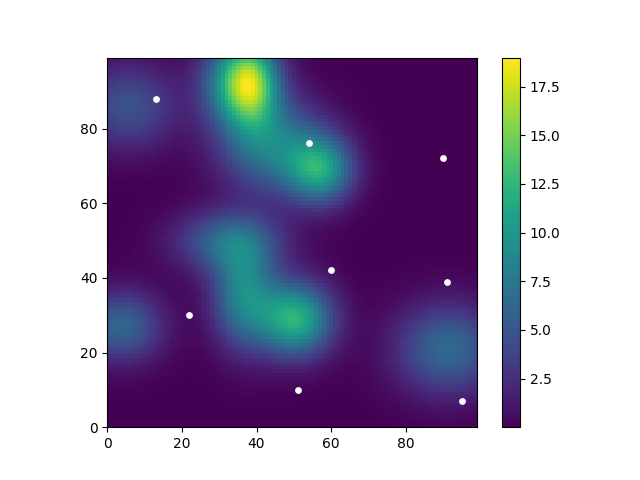
\includegraphics[width=\linewidth]{/home/rishab/Risk-Aware-TSP/plots/deterministic_info_path/info_map.png}
    \caption{}
  \end{subfigure}%
  \hspace*{\fill}   % maximize separation between the subfigures
  \begin{subfigure}{0.28\textwidth}
    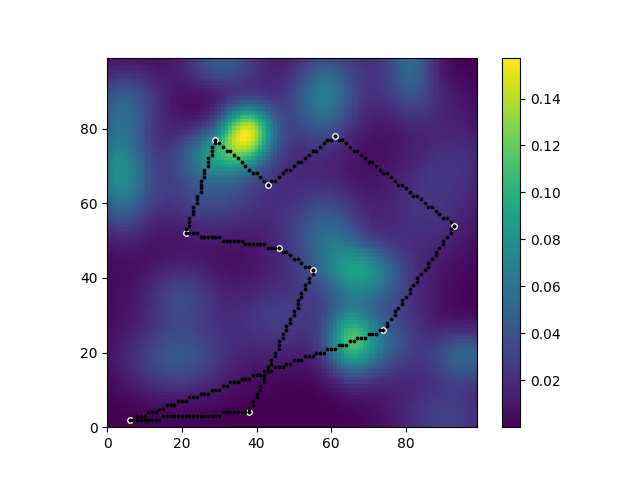
\includegraphics[width=\linewidth]{/home/rishab/Risk-Aware-TSP/plots/deterministic_info_path/path_alpha=0(pt)01.png}
    \caption{}
  \end{subfigure}%
  \hspace*{\fill}   % maximizeseparation between the subfigures
  \\
  
  \begin{subfigure}{0.28\textwidth}
    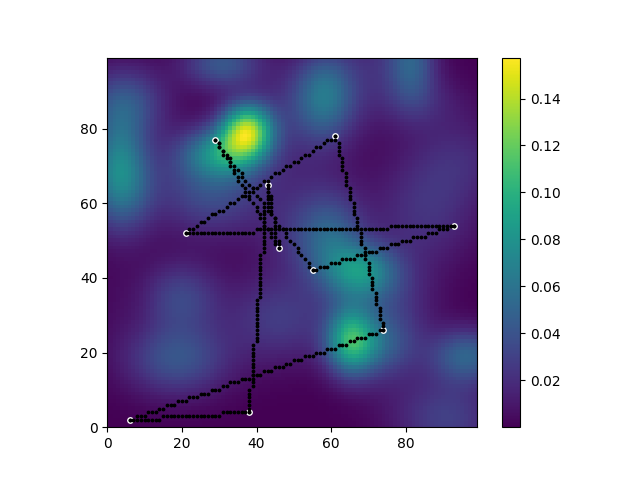
\includegraphics[width=\linewidth]{/home/rishab/Risk-Aware-TSP/plots/deterministic_info_path/path_alpha=0(pt)1.png}
    \caption{}
  \end{subfigure}%
  \hspace*{\fill}   % maximize separation between the subfigures
  \begin{subfigure}{0.28\textwidth}
    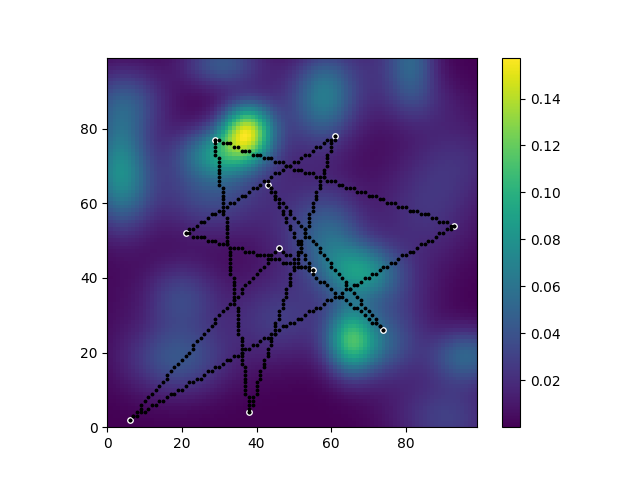
\includegraphics[width=\linewidth]{/home/rishab/Risk-Aware-TSP/plots/deterministic_info_path/path_alpha=0(pt)5.png}
    \caption{}
  \end{subfigure}%
  \hspace*{\fill}
  \\
  
  \begin{subfigure}{0.28\textwidth}
    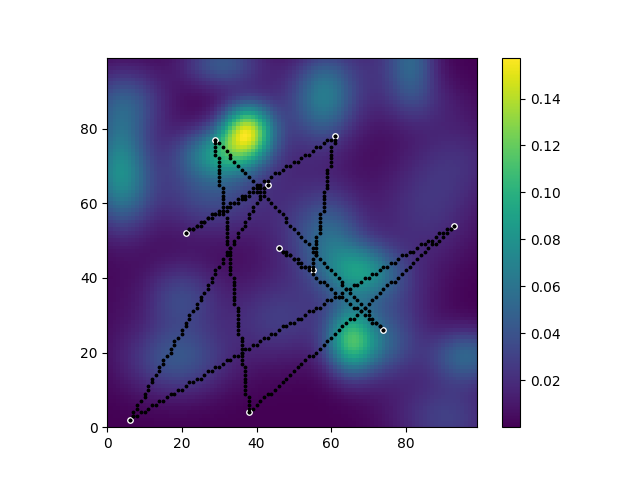
\includegraphics[width=\linewidth]{/home/rishab/Risk-Aware-TSP/plots/deterministic_info_path/path_alpha=0(pt)9.png}
    \caption{}
  \end{subfigure}%
  \hspace*{\fill}   % maximize separation between the subfigures
  \begin{subfigure}{0.28\textwidth}
    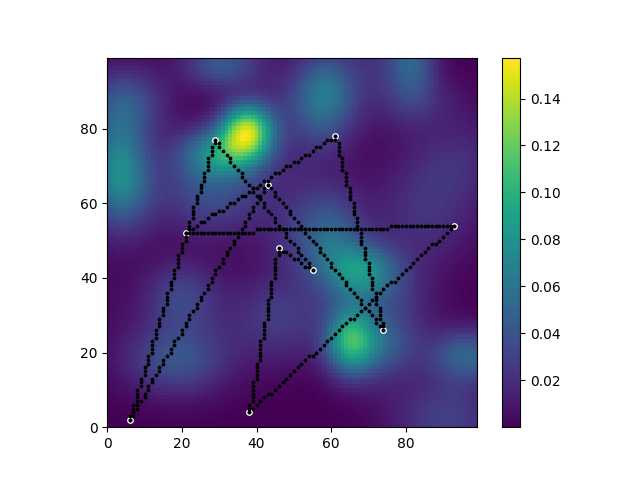
\includegraphics[width=\linewidth]{/home/rishab/Risk-Aware-TSP/plots/deterministic_info_path/path_alpha=1.png}
    \caption{}
  \end{subfigure}%
  \hspace*{\fill}
\caption{}
\end{figure}


\begin{figure}
\begin{center}
\begin{subfigure}{0.5\textwidth}
    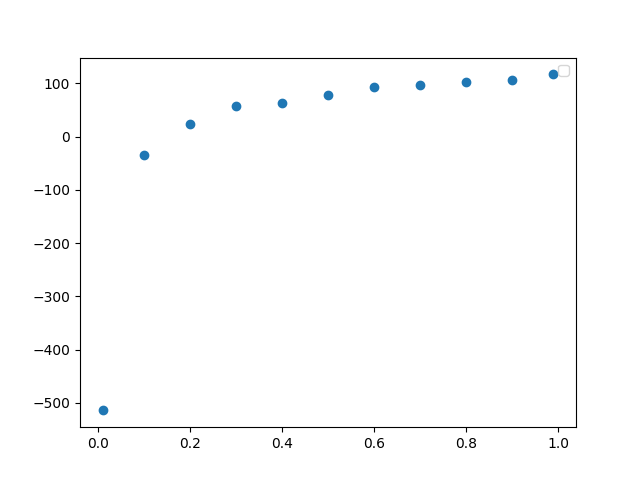
\includegraphics[width=\linewidth]{/home/rishab/Risk-Aware-TSP/plots/deterministic_info_path/H_vs_tau.png}
    \caption{}
  \end{subfigure}%
\end{center}
  \hspace*{\fill}   % maximize separation between the subfigures
  \\
  \begin{center}
   \begin{subfigure}{0.5\textwidth}
    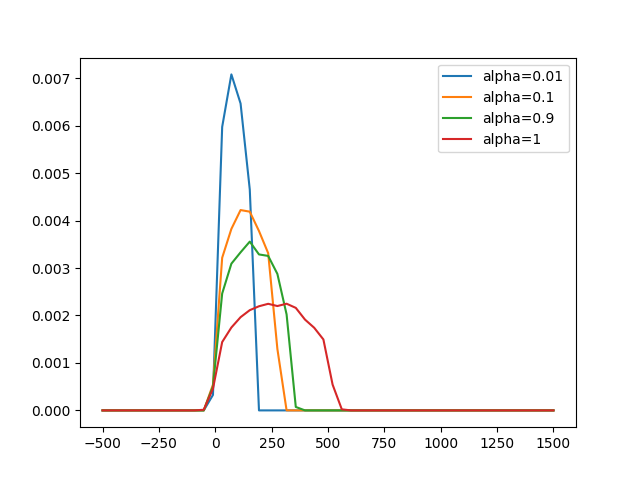
\includegraphics[width=\linewidth]{/home/rishab/Risk-Aware-TSP/plots/deterministic_info_path/Histogram.png}
    \caption{}
  \end{subfigure}%
  \end{center}
  \hspace*{\fill}   % maximizeseparation between the subfigures
\caption{}
\end{figure}

\section{Next To Do}
Point discussed
\begin{itemize}
    \item Implementation of stochastic risk for edges in graph $G(V,E)$, based on the Travelling Salesman formulation. We want to generate a Hamiltonan path with maximum reward given the expected risk along each edge (CVaR), and the operator threshold ($\alpha$).  
    
    \item Problem: $\max$ CVaR$_\alpha$ [w(S)], $s \in H$ 

    \item Each edge reward is a random variable, e.g., $r_{eij} ~ N(10, 2)$
    
    \item Solution: CVaR minimization with greedy TSP as subroutine 
    

\item Adding to the above algorithm costs, defined by constraints such as distance/fuel/time. These costs are deterministic. 

\item Altering the costs to be expectations of stochastic values, and improving the above algorithm
\end{itemize}

\section{Conclusion and Future Work}



\end{document}
